\documentclass[a4paper,10pt]{article}
\usepackage{graphicx}
\usepackage{verbatim}
\usepackage{subfig}
\usepackage{float}
\usepackage[spanish]{babel}   %ver bien como es
\usepackage[utf8]{inputenc}

\begin{document}

\tableofcontents

\newpage


\section*{Introducci\'on}
\addcontentsline{toc}{section}{Introducci\'on}

El objetivo de este trabajo es brindar posibles soluciones para el desarrollo de un software, el mismo ser\'a utilizado en una cadena de pizzer\'ias llamada "Pizza Hack". El análisis del software a desarrollarse fue solicitado por la cadena, que además puntualizó determinados objetivos que de antemano consideran importantes.


En conjunto con las explicaciones en lenguaje natural se incluyen modelos de objetivos y de agentes. Estos modelos permiten plasmar sintéticamente, de manera gráfica, una idea general de las características que identificamos en el conjunto de las posibles soluciones y que a su vez describen el problema. 

Una de las ventajas de los modelos de objetivos es que permiten identificar las relaciones entre los distintos objetivos de alto nivel, como así también descomponerlos en objetivos más concretos. Ésta descomposición permite a su vez delegar la responsabilidad del cumplimiento de un objetivo en una entidad activa, que se denomina agente, permitiendo de esta manera desarrollar soluciones alternativas con diferente grado de intervención del software en sí. Las alternativas que se generen a partir de la exploración de las posibles soluciones también se podrán ver representadas en forma esquemática. 

En los diagramas de contexto se podrán explorar con más detalle las interacciones que se darían en algunas de las variantes de nuestras posibles soluciones y entender mejor el rol que cumple cada agente.

De acuerdo a los objetivos priorizados por la cadena, el sistema debe tener las siguientes características:


El sistema pedido debe ser un sistema distribuido, es decir, debe operar en cada local por separado. Para realizar este an\'alisis para el posterior desarrollo del sofware se debi\'o pensar en que dicha cadena pretende ofrecer a sus clientes un men\'u en com\'un en todos los locales, es decir, mismo plato y mismo precio. Dicho men\'u debe poder ser modificado, por ejemplo si se desea cambiar alg\'un precio y agregar o quitar alguna variedad de pizza. Por otro lado, el sistema a desarrollar debe poder tener un manejo del nivel de stock, para que se pueda saber cuando se tienen que reponer los ingredientes. Adem\'as, conocer la cantidad de los elementos necesarios para realizar cada variedad que hay al momento, permite saber si un pedido va a poder ser realizado o no, de esta forma se garantiza que no se cancelen pedidos por falta de ingredientes. En el caso de que el cliente quiera pedir una variedad de pizza que no se pueda realizar en el local donde la est\'a pidiendo, se tiene que poder saber si en alg\'un otro local de la cadena hay stock como para realizar dicho pedido y contar con la posibilidad de reservar los ingredientes, al menos hasta que el cliente la retire en el otro local en cuestion. En el caso de que el cliente no pase a retirar el pedido se tiene que poder recuperar los ingredientes reservados. Finalmente, este informe brinda el an\'alisis de dicho software y requerimientos del hardware para el sistema.
\\
\textbf{Cosas que dijo la catedra: acá debería figurar todo lo necesario como para que un lector no iniciado en el tema entienda el propósito general del sistema que van a describir. Puede citar algunos fragmentos del enunciado si lo consideran necesario, pero NO DEBE SER una copia del enunciado.}

\newpage
\section*{Presunciones}
\addcontentsline{toc}{section}{Presunciones}
En esta secci\'on se describen las cosas que se asumen que no pueden pasar o que pasan.\\
\textbf{Cosas que dijo la catedra: acá deberían listar aquellas cuestiones que asumieron por encima del enunciado. Estas cuestiones pueden provenir de alguna consulta con docentes. También pueden provenir de alguna especulación o interpretación que el grupo hizo.}
\\

\noindent
\textbf{Tiempo de pedido:} asumimos que dos clientes no puede hacer un pedido de forma simultánea. Esta presunción permite simplificar el cumplimiento del objetivo relacionado a no dejar que se pueda cancelar un pedido a un cliente luego de que fue hecho, dado que establece un claro orden entre ellos. \\
\textbf{Tiempo de pedido a distancia:} asumimos que, ante un pedido a `distancia' (es decir, de un local a otro), un cliente pierde el interés en buscar dicho pedido luego de un \textit{time out} pautado de antemano. Esta presunción nos ayuda a poder cumplir, por un lado, el objetivo relacionado a permitir dicha compra `a distancia' y, por otro, a poder mejorar el manejo de stock al cancelar el pedido luego de pasado el \textit{time out}, y de esta forma recuperar el stock reservado para éste. Esto se logra sin violar los objetivos relacionados al funcionamiento de las ventas (no cancelar pedidos hechos), dado que se interpreta como que el cliente es el que cancela el pedido al no presentarse y no el local.\\
\textbf{No hay actualizaciones simultáneas:} Habiéndose hecho especial énfasis en que la solución informática no debe ser centralizada, en caso de haber actualizaciones simultáneas se debería arbitrar, de manera distribuída, cuál de las actualizaciones es la que corresponde propagar a la totalidad de las sucursales. Siendo ésta una situación que no consideramos muy común, parece razonable suponer que no hay actualizaciones simultáneas de las variedades del menú. De ésta manera dicho arbitraje no es necesario. \\ 
\newpage
\section*{Vistas}
\addcontentsline{toc}{section}{Vistas}

\textbf{Cosas que dijo la catedra: está sería la parte principal del TP. Acá irían los diagramas y los escenarios representativos de uso. No necesariamente tiene que ser una gran sección, sino que pueden partirla por funcionalidades y a su vez por tipo de vista o de la forma que crean más pertinente. Esta sección NO DEBE SER una simple seguidilla de figuras sueltas. Debe estar acompañada de tantas explicaciones como sean necesarias para que se aprecie un hilo conductor.}

\section*{Diagrama de contexto}
\section*{1}
El siguiente diagrama de contexto muestra los agentes involucrados en interacciones con una solución que se orienta a la automatización. 

\paragraph{Proveedor:}
El proveedor es el encargado de reponer el stock a pedido de nuestro local. Incluye todo el sistema de compra y transporte de productos hasta el local.
\\
\paragraph{Menú Electrónico:}
El menú electrónico consiste en un menú interactivo ofrecido a los usuarios a través de iPADs, los cuales son asignados de a uno por mesa. En éste pueden distinguirse las distintas variedades de productos (no únicamente pizzas, sino también bebidas y postres) y sus correspondientes precios. A su vez, en distintos colores se puede distinguir si el producto está o no disponible (es decir, si hay stock de ingredientes para preparalo) y si, en caso de que no haya, puede o no ser pedido en otro local en que sí haya stock, ofreciéndo al cliente la opción de elegir en qué local puede hacer el pedido.
\\
\paragraph{Cliente:}
El cliente que entra al local. Se refiere tanto a individuos como a grupos.
\\
\paragraph{Personal:}
Se refiere al conjunto de personas que trabajan en el local, éstos son: los mozos, el cajero y los cocineros.
\\

La solución presentada en general prioriza la satisfacción del cliente, ya que al ocuparse el software de manera casi íntegra del manejo de stock, resulta posible descontar inmediatamente la disponibilidad de un determinado ingrediente al registrarse un pedido, incluso antes de iniciarse su preparación. Esto evita que al ocurrir varios pedidos concurrentes se acepten pedidos para los cuáles no se dispone de stock suficiente.

Por otra parte, aún cuando el personal no hubiera registrado la escacez de un ingrediente, el sistema lo informaría logrando la reposición del mismo. Debido a posibles imprecisiones en las cantidades de ingredientes registradas para cada receta es necesario que el personal periódicamente haga un inventario completo de las existencias y actualice las cantidades disponibles mediante una interfaz gráfica que será provista por el software.

Es importante destacar que en este caso estamos considerando la comunicación entre sucursales parte del sistema a desarrollarse. En este sentido este sistema no es completamente tolerante a fallas, ya que en el caso de falla por parte del proveedor de servicio de Internet, el sistema se vería inhabilitado para realizar operaciones entre sucursales. Se podría agregar un modo de funcionamiento manual, pero no garantizaría los beneficios del sistema automatizado y además agregaría costo en concepto de funcionalidades que sólo se utilizarían en caso de falla total del servicio de Internet. 
\begin{figure}[H]
\centering
\subfloat{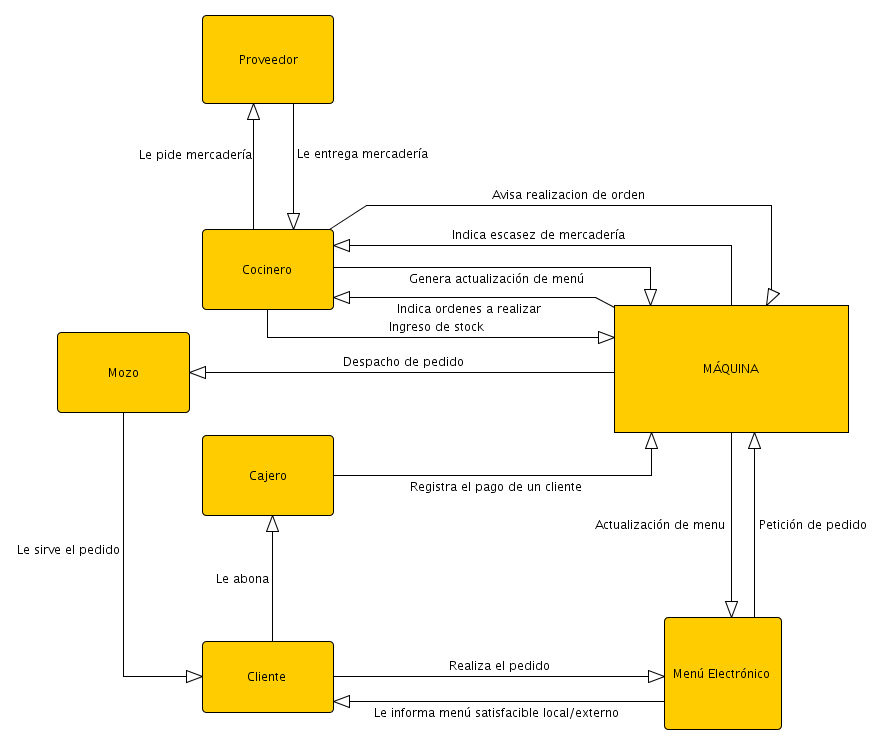
\includegraphics[width=1.2\textwidth]{imagenes/agentes_automatico.png}}
\caption{Diagrama de contexto orientación automatización.}
\end{figure}

\section*{2}
El siguiente diagrama de contexto muestra los agentes involucrados en interacciones con una solución que se orienta a la automatización. 
El siguiete diagrama de contexto muestra los agentes involucrados en la interaccion con una solucion orientada a mecanismos manuales


\paragraph{Proveedor:}
El proveedor es el encargado de reponer el stock a pedido de nuestro local. Incluye todo el sistema de compra y transporte de productos hasta el local.
\\
\paragraph{Personal:}
Se refiere a todo el conjunto de personas empleadas en el local. El conjunto tiene una gran interacción con la maquina y con el cliente dado que debe cumplir varias funciones. Actualizar nivel de stock, cuando se hace una nueva compra debe registrarse el cambio. Debe ingresar un pedido al sistema (proveniente de un cliente) para que este evalue si puede o no satisfacerlo. Debe registrar el pago de un cliente. Recibe la confirmación de satisfacción por parte del software, que le indica que puede confirmarle el pedido a un cliente. Tiene también la tarea de pedir al proveedor lo que haga falta corroborando el estado del stock. Debe llevar/recibir/confirmar/servir un pedido.Tiene el deber de actualizar el menu cuando lo crea pertinente.
\\
\paragraph{Cliente:}
Se refiere al conjunto de personas que trabajan en el local, éstos son: los mozos, el cajero y los cocineros.
\\
\paragraph{Menu impreso:}
En esta familia de soluciones, contamos con un menu impreso que debe ser actualizado en todo momento para seguir siendo consistente con la realidad. Cada vez que se quiere actualizar debe ser reeimpreso.
\\
\paragraph{Motopizza:}
Sistema de humanos de altacomplejidad encargado de realizar diversas tareas. Debe encargarse de actualizar los datos que vienen de afuera, para esto recorre todas las demas sucursales (lo que puede actualizar con, cambios de menu y peticiones de pedidos) Ademas debe recorrer pizzerias para informar que va un cliente si es posible y propagar el menu local. Ese sistema es sumamente ineficiente.

\begin{figure}[H]
\centering
\subfloat{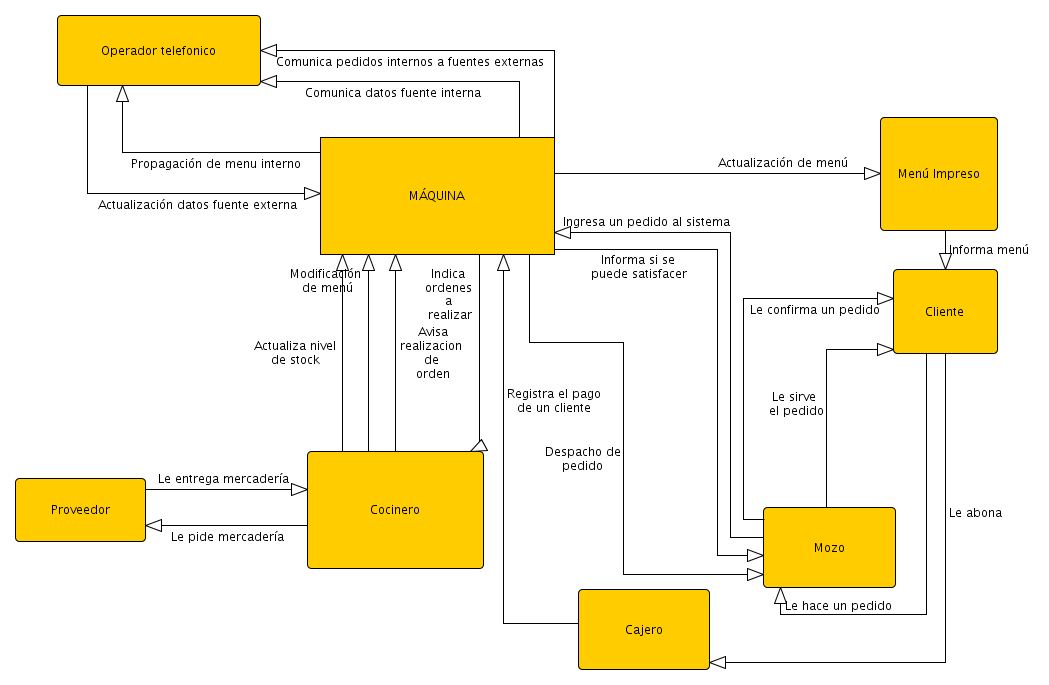
\includegraphics[width=1.2\textwidth]{imagenes/agentes_manual.png}}
\caption{Diagrama de contexto orientación automatización.}
\end{figure}

\section*{3} Podemos armar distintos tipos de diagramas de contexto apartir de estos dos, dado que presentan opciones para cosas distintas tambien. Ej, se podria poner un menu electronico y trabajar con el Motopizza. O también usar sistema de comunicaciones sofisticado con un menu impreso. Se pueden ir armando distintas combinaciones.


\section*{Modelo de objetivos}
\addcontentsline{toc}{subsection}{Modelo de objetivos}

%\centering
%\includegraphics[scale=0.5]{TP1 - Modelo de objetivos - Parte I.png}

\subsection*{Objetivos}
\addcontentsline{toc}{subsubsection}{Objetivos}
\noindent

El siguiente diagrama expresa algunos de los objetivos requeridos por la cadena y que consideramos troncales.

\begin{figure}[H]
\centering
\subfloat{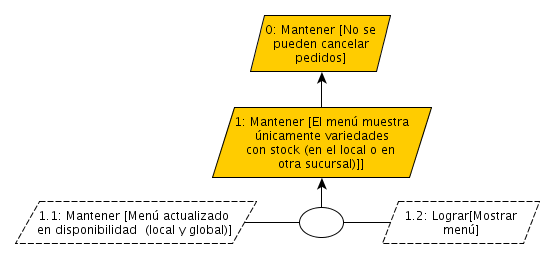
\includegraphics[width=1.3\textwidth]{imagenes/objetivos_principales.png}}
\caption{Objetivos principales}
\end{figure}

Los objetivos planteados garantizan que un pedido no será cancelado una vez confirmado. Es decir, un pedido no será cancelado por falta de ingredientes para prepararlo. 

Para lograr esto proponemos que el menú sólo muestre variedades de pizza disponibles, ya sea en la sucursal en la que se está consultando el menú, o eventualmente en otra sucursal, obviamente indicando dicha particularidad.

El objetivo de mantener el menú actualizado en cuanto a disponibilidad plantea a su vez varios objetivos relacionados, por lo que a continuación nos extendemos en su descripción.

\begin{figure}[H]
\centering
\subfloat{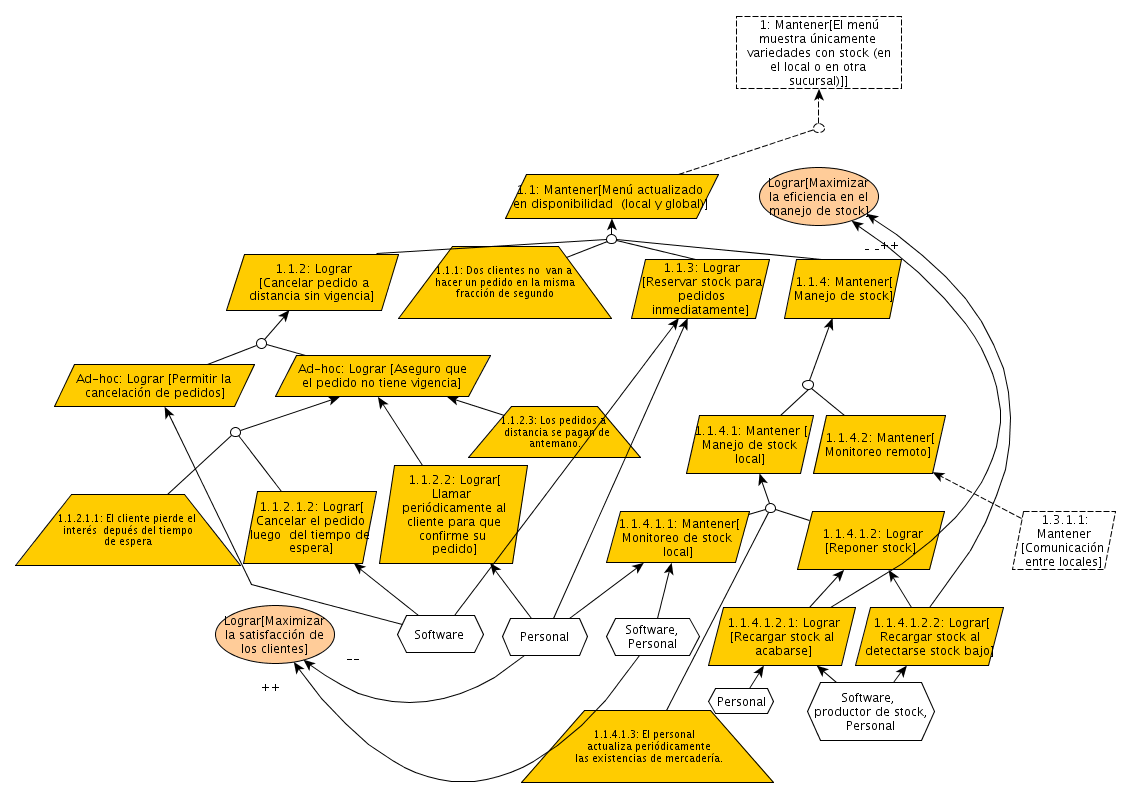
\includegraphics[width=1.3\textwidth]{imagenes/objetivos_menu.png}}
\caption{Objetivos principales}
\end{figure}

Como se puede apreciar, surge una gran cantidad de objetivos en algún sentido más simples, algunos de los cuáles consideramos que pueden ser concretados por un agente en particular. En estas asignaciones de objetivos van a surgir las diferentes variantes de la solución propuesta. 

En el anterior diagrama se muestra una dependencia entre el objetivo 1.1 y el 1.1.4. Estrictamente parecería que lo único que es relevante al objetivo 1.1 con respecto al manejo de stock es el monitoreo, tanto local, o restringido a la sucursal en la que se usa el menú, como global, o remoto, del mismo. Por cómo pensamos la solución de software, esta dependencia en realidad existiría, ya que el manejo de stock estaría intimamente ligado a la exactitud y actualidad de los datos obtenidos mediante el monitoreo. Es por eso que mantenemos esa jerarquía.


A continuación nos enfocaremos en el objetivo 1.1.4.1.1. 
\subsubsection*{Mantener [Monitoreo de stock]}
Como vemos, consideramos que existe la opción de asignar la concreción de este objetivo por un lado al Personal, y por otro al Software en conjunto con el Personal. Esta apreciación merece algunas observaciones.
En primer lugar, asignarlo al Personal consistiría en que los cocineros actualicen con cada pedido el stock disponible, descontando manualmente, mediante una interfaz provista por el software, los ingredientes utilizados en cada caso.  


La opción de asignarlo al Software en conjunto con el Personal consiste en que el software asocie cada variedad de pizza a los ingredientes, con sus cantidades correspondientes, necesarios para prepararla. De esta manera, en el instante mismo en que se genera un pedido, el sistema actualizaría las cantidades disponibles de cada ingrediente de manera automática y sin intervención del personal. Sin embargo, por no ser exactas las cantidades registradas en la receta, sería necesario que el Personal haga un inventario completo periódicamente y actualice la disponibilidad de ingredientes con los valores reales.

En este sentido, la expectativa 1.1.4.1.3 tiene varias implicaciones. En el caso de cumplir el objetivo 1.1.4.1.1 con una solución mixta, el Personal debería actualizar las existencias con una periodicidad dada por la eventual inexactitud de las recetas. En el caso de cumplirlo sólo mediante la participación del Personal, sería necesario que la actualización de las existencias fuera casi permanente.

La decisión respecto del objetivo 1.1.4.1.2 está relacionada con las consideraciones mencionadas, ya que, en caso de tenerlo, sería deseable aprovechar las capacidades de monitoreo de stock provistas por el software para alertar al personal de manera que realice un pedido al proveedor si fuera necesario. Las dos políticas de recarga de stock son mencionadas debido a que, si bien la recarga de stock al acabarse es mejor en relación a maximizar la eficiencia en el manejo de stock, ya que se realiza un pedido de mercadería sólo cuando es necesario, es claramente deficiente en relación a la satisfacción del cliente, ya que permite que haya variedades de pizza no disponibles.


La realización de pedidos a distancia, reservando el stock necesario para prepararlo, está relacionada con la precisión del monitoreo de stock. Por lo que ahora nos centraremos en el objetivo 1.1.2:
\subsubsection*{Lograr [Cancelar pedido a distancia sin vigencia]}
Como mencionamos, al realizar un pedido a distancia, los ingredientes para realizar dicho pedido deben ser reservados, garantizando de esa manera que, al llegar el cliente a la sucursal, su pedido todavía puede realizarse. El conflicto surge si un cliente pierde el interés en su pedido y no lo va a retirar.
Este objetivo trae aparejados varios obstáculos, ya que en principio se desearía evitar cancelar un pedido excepto en casos en los que se pudiera asegurar que el cliente perdió el interés en su pedido, pero por otra parte, no es deseable que se mantengan reservados ingredientes que no van a ser utilizados.
Las opciones que a continuación detallamos tienen cada una sus propias ventajas y desventajas, por lo que eventualmente sería necesario que un experto de dominio aporte más información.


Una forma de resolver este conflicto es asumir que los clientes nunca van a retirar su pedido pasado cierto tiempo, debido a que pierden el interés. Siguiendo este razonamiento es seguro volver a disponer de los ingredientes reservados. La limitación de este enfoque es la falta de flexibilidad, ya que un cliente podría retrasarse mucho más de lo común y aún así pasar a buscar su pedido luego de un tiempo considerable.

Una sofisticación de esta idea es requerir información de contacto al realizar un pedido a distancia, un teléfono celular por ejemplo. Y periódicamente llamar al cliente para confirmar que mantiene su interés, dando de baja el pedido en caso contrario. Esta opción, mucho más flexible que la anterior, requiere la participación del Personal y por otra parte requiere que los clientes provean algún tipo de medio de contacto para tener alguna utilidad.

Por último, si los clientes pagaran su pedido en la sucursal en la que se encuentran, aún si el mismo se entregara en otra, sería razonable suponer que lo va a pasar a buscar, por lo que no habría pedidos a distancia que perdieran la vigencia y no sería necesario cancelarlos.

Más adelante retomaremos el objetivo 1.3.1.1, referido a la comunicación entre locales.
El resto de los objetivos tienen nombres lo suficientemente explicativos, por lo que vamos a retomar los objetivos planteados por la cadena.

\begin{figure}[H]
\centering
\subfloat{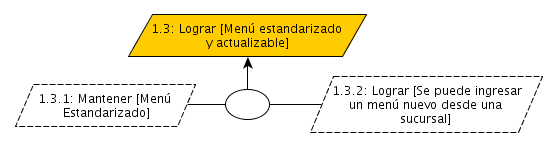
\includegraphics[width=1.3\textwidth]{imagenes/objetivos_menu_estandarizado.png}}
\caption{Objetivos principales}
\end{figure}

Entre las pautas se menciona la necesidad de poder actualizar el menú y la restricción de que el menú sea el mismo para todas las sucursales. A continuación nos enfocamos en el objetivos 1.3.1:
\subsubsection*{Mantener [Menú estandarizado]}
para mantener un menú estandarizado simplemente tenemos que aseguranos que sea el mismo en todos los locales, sean cual sean las actualizaciones que se han realizado (de variedades, precios, etc). Para ello únicamente tenemos que asegurar que se mantenga la comunicación entre los locales. \\
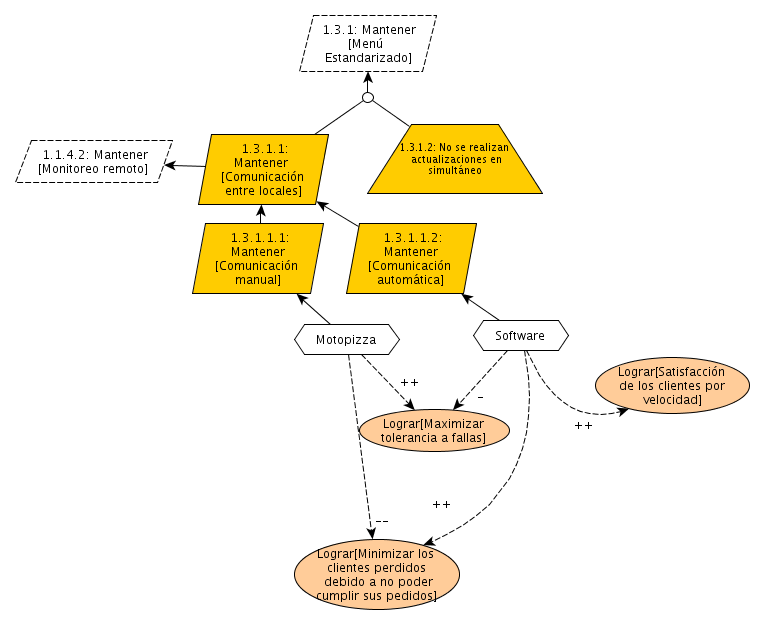
\includegraphics[width=400pt]{imagenes/objetivos_menu_estandarizado2.png}


La presunción 1.3.1.2 es explicada en mayor detalle en la sección de presunciones.
Las opciones mediante las cuales se puede lograr el objetivo 1.3.1.1 consisten en establecer manualmente la comunicación, entre sucursales o dejarla en manos del software, que operaría a través de internet. 

La opción manual consiste en delegar la tarea de mantener la comunicación a un miembro del Personal, distinguido por su movilidad a través de una moto. Su versatilidad le permite adaptarse a muy variadas situaciones, por ejemplo, en el caso general, con sólo comunicarse telefónicamente le alcanzaría, pero ante una falla en este servicio, podría trasladarse a cada una de las sucursales restantes informando novedades y a la vez recibiéndolas. 

Por supuesto, esta solución tiene como defecto principal la velocidad. No se puede, de esta manera, suponer que la información que tenemos de las otras sucursales es absolutamente actualizada, por lo que podrían ocurrir algunos conflictos debidos a este retraso en la transmisión de información. Como ejemplo de esto, ante el pedido de una variedad que se consideraba disponible en uns sucursal remota, este sería autorizado, para luego verificar que la información de la que se disponía era desactualizada. 
Una de las razones que nos hizo considerar la opción manual es su superioridad en términos de tolerancia a fallas. Si esto resulta una característica importante, sería conveniente considerar esta posibilidad.

La solución mediante software ofrece una menor tolerancia a fallas, pero en el caso general garantiza una mayor satisfacción del cliente en cuanto a velocidad, ya que los tiempos de comunicación son mínimos, permitiendo gestionar pedidos a distancia instantaneamente y garantizar que la información compartida es efectivamente la más reciente.

También se da un mejor trato a los clientes, ya que al contar con información actualizada se puede indicar al cliente donde conseguir su variedad preferidad garantizando la no cancelación de su pedido. Esto aporta positivamente a su satisfacción.


%Se debera permitir aceptar pedidos de una sucursal remota y a la vez poder realizar los pedidos que no sean satisfechos pro el local en cuestion a otra sucursal de la cadena que si disponga del stock necesario para cubrir el pedido del cliente.

Para terminar de asegurar la concreción del objetivo 1.3 ahora nos remitimos al objetivo 1.3.2:
\subsubsection*{Lograr [Se puede ingresar un menú nuevo desde una sucursal]}

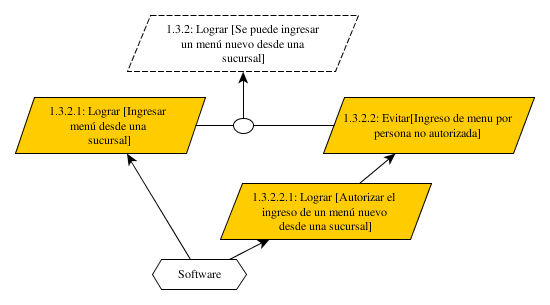
\includegraphics[width=400pt]{imagenes/objetivos_menu_ingreso.png}

\newpage
\section*{Escenarios}
El dia 29/02/2004 a las 12:47:59 entran simultaneamente al local de pizza Hack (sucursal barrio mitre) Alan Faina, 
Sergio Mazza, Tom\'as Anchorena y Laura Oliva en busqueda de una buena sapi. 
Alan se sienta en la mesa nro 1, Tomas en la mesa nro 2, Sergio Mazza en la 3 y Laura Oliva en la mesa 4. 

Alan se dispone a pedir su pizza preferida, la de anchoas, toma entonces el men\'u electr\'onico que se encuentra sobre su mesa y
mediante la secuencia de botones Comidas $\rightarrow$ Pizzas $\rightarrow$ Anchoas efectiviza su pedido y queda a la espera del mismo. El pedido se pudo 
realizar porque el monitereo de stock indicaba que la cantidad de anchoas era suficiente para realizar la pizza y, por lo tanto, en el men\'u
esta opci\'on le aparec\'ia a Alan como elegible. Sin embargo, el stock presente solo alcanzaba para una pizza de anchoas, por lo que (el agente
que moniterea el stock) le avisa al personal de la pizzeria que es hora de comprar m\'as anchoas.

Mientras tanto, en la mesa 2, Tomas Anchorena tambi\'en se dispone a pedir su pizza favorita que, al igual que Alan, se trata de la pizza de 
anchoas. Sin embargo, siendo Tomas tan pulcro, no postergo el lavado de sus manos por lo que cuando volvio a su mesa, Alan ya habia realizado
su pedido. Cuando entonces Tomas se dispone a pedir su ansiada pizza de anchoas, comienza a tocar la misma secuencia de botones que Alan. Sin embargo
cuando entra al men\'u de pizzas, se encuentra que el bot\'on correspondiente a la pizza de anchoas esta en gris (es decir, que no es seleccionable).
Tomas, desesperado por su pizza y conociendo el men\'u electr\'onico de la afamada pizzer\'ia, se fija si su pizza se encuentra disponible en otro
local. Pero, al igual que el bot\'on anterior, el bot\'on que indica la opci\'on para pedir pizza en otra sucursal, tampoco se encuentra disponible.

Tom\'as se retir\'a del local, triste por su pizza de anchoas, pero ya haciendosele agua la boca por la fugazzeta rellena de Banchero, su proxim\'o destino.

 
\begin{itemize}
\item pedir en otra sucursal e ir
\item pedir en otra y no ir
\item faltaria pedir stock
\end{itemize}

%El dia 29/02/2004 a las 12:47:59 entran simultaneamente al local de pizza Hack (sucursal barrio mitre) Alan Faina, Sergio Mazza, Tomas Anchorena y 4taPersona en busqueda de una buena sapi. Alan se sienta en la mesa nro 1, tomas en la mesa nro 2, sergio mazza en la 3 y la 4ta en la mesa 4. 
%\begin{itemize}\item
%\item pedir en otra sucursal e ir
%\item peidr en otra y no ir
%\item pedir y que no haya
%\item pedir y que haya y que el siguiente no tenga
%\item que se quede sin stock y pedir stock.
%\end{itemize}

\newpage
\section*{Discusi\'on}
\addcontentsline{toc}{section}{Discusi\'on}

\textbf{Cosas que dijo la catedra: debe contener un análisis general de las distintas alternativas y su impacto en los objetivos blandos. NO DEBE SER una lista de lo que ya se puede desprender del diagrama. Debe ser un análisis más cualitativo y "a vuelo de pájaro" que permita entender este asunto en pocas palabras. Esta sección también es ideal para quevuelquen las cosas que puedan haberles quedado "flojas" o no cerradasdel todo: por ejemplo los potencia les conflictos entre objetivos, los aspectos que podrían hacer que todo el sistema no funcione como desean, etc.}
Para la resoluci\'on de este sistema se presentaron distintas alternativas contemplando diversos presupuestos. Las soluciones propuestas son las siguientes:
\begin{itemize}
\item Local manual: se basa en que haya mozos que presenten el men\'u de forma oral.
\item Local automatizado: se basa en brindar en cada mesa un men\'u electronico.
\item Local mixto: se basa en una mezcla entre el manual y el automatizado, es decir, que en la caja haya un men\'u electronico que es presentado por mozos en cada mesa.
\end{itemize}


\newpage
\section*{Conclusiones}
\addcontentsline{toc}{section}{Conclusiones}

\textbf{Cosas que dijo la catedra: mencionar brevemente de qué formas les resultó más sencillo encarar el TP. Por ejemplo en qué orden realizaron los diagramas, qué aspectos presentaron las mayores dificultades, etc.}




\end{document}
